%%%%%%%%%%%%%%%%%%%%%%%%%%%%%%%%%%%%%%%%%%%%%%%%%%%%%%%%%%%%%%%%%
%%% %
%%% % weiiszablon.tex
%%% % The Faculty of Electrical and Computer Engineering
%%% % Rzeszow University Of Technology diploma thesis Template
%%% % Szablon pracy dyplomowej Wydziału Elektrotechniki 
%%% % i Informatyki PRz
%%% % June, 2015
%%%%%%%%%%%%%%%%%%%%%%%%%%%%%%%%%%%%%%%%%%%%%%%%%%%%%%%%%%%%%%%%%

\documentclass[12pt,twoside]{article}

\usepackage{weiiszablon}
\usepackage{fancyhdr}
\usepackage{amsmath}
\usepackage{graphicx}
\usepackage{graphicx}
\usepackage{subcaption}
\usepackage{verbatim}

\fancyhf{} % Wyczyść bieżące ustawienia stopki
% Ustawienia dla lewego rogu stopki
\fancyfoot[L]{D.K.}

% Ustawienia dla prawego rogu stopki
\fancyfoot[R]{\thepage}


\author{Daniel Kleczyński}

% np. EF-123456, EN-654321, ...
\studentID{XX-??????}

\title{Model neuronu oraz pojedyncze iwielowarstwowe sieci neuronowe }
\titleEN{Temat pracy po angielsku}


%%% wybierz rodzaj pracy wpisując jeden z poniższych numerów: ...
% 1 = inżynierska	% BSc
% 2 = magisterska	% MSc
% 3 = doktorska		% PhD
%%% na miejsce zera w linijce poniżej
\newcommand{\rodzajPracyNo}{0}


%%% promotor
\supervisor{dr hab. inż. Roman Zajdel, prof. PRz}
%% przykład: dr hab. inż. Józef Nowak, prof. PRz

%%% promotor ze stopniami naukowymi po angielsku
\supervisorEN{(academic degree) Imię i nazwisko opiekuna}

\abstract{Treść streszczenia po polsku}
\abstractEN{Treść streszczenia po angielsku}

\fancyhf{} % Wyczyść bieżące ustawienia stopki
% Ustawienia dla lewego rogu stopki
\fancyfoot[L]{D.K.}

% Ustawienia dla prawego rogu stopki
\fancyfoot[R]{\thepage}

\begin{document}




\author{L8 2EF-DI \\ Daniel Kleczyński}

% strona tytułowa
\maketitle



% spis treści
\tableofcontents

\clearpage



\section*{Wprowadzanie}
\addcontentsline{toc}{section}{Wprowadzanie}%
Rozwiązania oparte na modelach neuronów i sieciach neuronowych, zaliczają się do alghorytmów uczenia maszynowego, mają szerokie zastosowanie jako iteracyjne
metody uczenia. Oznacza to, że w procesie uczenia modelu sieci neuronowej, wagi połączeń między neuronami są dostosowywane iteracyjnie na podstawie analizy i porównania wyników predykcji z oczekiwanymi wartościami.

Algorytmy oparte na modelach neuronów i sieciach neuronowych znajdują zastosowanie w wielu obszarach:

Klasyfikacja: Sieci neuronowe mogą być wykorzystywane do klasyfikacji danych, czyli przypisywania nowych obserwacji do odpowiednich
kategorii na podstawie wcześniej nauczonych wzorców. Przykładem może być klasyfikacja obrazów na podstawie ich zawartości, rozpoznawanie
ręcznego pisma lub diagnozowanie chorób na podstawie analizy medycznych danych.

Aproksymacja: Sieci neuronowe mogą służyć do aproksymacji złożonych funkcji lub powiązań między danymi wejściowymi a danymi
wyjściowymi. Dzięki swojej zdolności do modelowania nieliniowych zależności, sieci neuronowe mogą być stosowane do prognozowania cen, analizy
rynkowej, predykcji wartości lub prognozowania trendów w danych.

Uogólnianie przypadków: Sieci neuronowe są również używane do uogólniania przypadków. Oznacza to, że po nauczeniu się na
podstawie dostępnych danych, sieć jest w stanie rozpoznać i odpowiedzieć na nowe przypadki, które nie były obecne w danych uczących.
Przykładem może być rozpoznawanie wzorców w danych sensorycznych lub klasyfikacja obiektów w obrazach.

Generowanie nowych treści: Sieci neuronowe, szczególnie rekurencyjne sieci neuronowe (RNN) i generatywne sieci adversarialne (GAN), mają
zdolność generowania nowych treści na podstawie wcześniej nauczonych wzorców. Przykładowe zastosowania to generowanie obrazów, tworzenie
tekstu lub generowanie muzyki.

Algorytmy oparte na modelach neuronów i sieciach neuronowych są wszechstronne i oferują wiele możliwości w dziedzinie uczenia maszynowego. Dzięki swojej zdolności do wykrywania i modelowania złożonych zależności, są one używane w wielu dziedzinach nauki, przemysłu i technologii.

\clearpage

\section{Model pojedynczego neuronu}

Model neuronu McCullocha-Pittsa, znany również jako model neuronu logicznego, jest jednym z najwcześniejszych modeli matematycznych neuronu. Został zaproponowany przez Warrena McCullocha i Waltera Pittsa w 1943 roku. Model ten opisuje prosty sposób działania pojedynczego neuronu jako jednostki przetwarzającej informacje.

W modelu McCullocha-Pittsa neuron przyjmuje binarne wartości wejściowe (0 lub 1) oraz posiada wagi odpowiadające połączeniom między wejściem a neuronem. Każde wejście jest mnożone przez odpowiadającą mu wagę, a następnie sumowane. Jeśli suma przekroczy pewien próg, neuron generuje wartość wyjściową (1), w przeciwnym przypadku generuje wartość (0). Model ten można opisać matematycznie jako:

Wyjście neuronu:
$$y = f(\sum_{i=1}^{n} w_i \cdot x_i)$$

gdzie:
\begin{itemize}
	\item $y$ to wartość wyjściowa neuronu (0 lub 1),
	      \item$x_i$ to wartość wejściowa i-tego połączenia,
	      \item$w_i $ to waga i-tego połączenia,
\end{itemize}
$y$ to wartość wyjściowa neuronu (0 lub 1),
$x_i$ to wartość wejściowa i-tego połączenia,
$w_i $to waga i-tego połączenia,
$f$ to funkcja progowa, która przekształca sumę na wartość wyjściową (np. 0 dla sumy < próg, 1 dla sumy >= próg).

Model McCullocha-Pittsa jest uproszczonym modelem neuronu, który nie uwzględnia nieliniowości ani uczenia. Nie pozwala na adaptację wag na podstawie dostępnych danych uczących. Niemniej jednak, ten model stanowił podstawę do dalszych rozwojów w dziedzinie sztucznych sieci neuronowych.

\subsection{Ćwiczenie I}

Dla pojedynczego neuronu o wagach [.1 .4 -.3 .7], przesunięcia [.5] i wektora sygnałów wejściowych [1 2
3 4] wyznaczyć łączne pobudzenie neuronu.

\begin{lstlisting}[language=Python,caption=Pierwotny sposób,label={KodPerl1}]
	w=np.array([.1, .4, -.3, .7])
	x=np.array([range(1,5)])
	b=.5
	z=w.dot(x.T)+b
	
\end{lstlisting}

\begin{lstlisting}[language=Python,caption=I sposób ,label={KodPerl1}]
	w = np.array([.1, .4, -.3, .7])
	x = np.array([1, 2, 3, 4])
	b = .5
	z = np.sum(w*x) + b
	
\end{lstlisting}
\begin{lstlisting}[language=Python,caption=II sposóbl,label={KodPerl1}]
	w = np.array([.1, .4, -.3, .7])
	x = np.array([1, 2, 3, 4])
	b = .5
	z = 0
	for i in range(len(x)):
		z += w[i]*x[i]
	z += b
	
\end{lstlisting}
\begin{lstlisting}[language=Python,caption=III sposób,label={KodPerl1}]
	w = np.array([.1, .4, -.3, .7])
	x = np.array([1, 2, 3, 4])
	b = .5
	z = np.sum(np.multiply(w, x)) + b
	
\end{lstlisting}

\subsection{Ćwiczenie II}
Zapoznać się z funkcjami przejścia neuronu: $hardlim$, $hardlims$, $purelin$, $satlin$,
$satlins$, $logsig$, $tansig$, $radbas$. Wykorzystując definicje funkcji zawarte w dodatku I
narysować wykresy funkcji przejścia neuronów dla łącznego pobudzenia z przedziału od -10 do 10.
W sprawozdaniu zamieścić ich wykresy i programy rysujące.Na prośbę prowadzącego napisać własną implementacje funkcji aktywacji


\begin{lstlisting}[language=Python,caption= Implementacja funkcji aktywacji , label={KodPerl1}]

	def hardlim(x):
	    return np.where(x>=0, 1, 0)

	def hardlims(x):
	    return np.where(x>=0, 1, -1)

	def purelin(x):
	    return x

	def satlin(x):
	    return np.where(x>=1, 1, np.where(x<=0, 0, x))

	def satlins(x):
	    return np.where(x>=1, 1, np.where(x<=-1, -1, x))

	def logsig(x):
	    return 1 / (1 + np.exp(-x))

	def tansig(x):
	    return np.tanh(x)

	def radbas(x):
	    return np.exp(-(x**2))

\end{lstlisting}




Funkcje aktywacji są kluczowym elementem w modelach neuronowych, ponieważ wprowadzają nieliniowość i umożliwiają modelowanie bardziej skomplikowanych zależności między danymi wejściowymi a wyjściowymi. Oto krótkie opisy kilku funkcji aktywacji przedstawionych w Twoim kodzie:

\begin{align*}
	\text{hardlim}(x) &= \begin{cases}
	1, & \text{dla } x \geq 0 \\
	0, & \text{dla } x < 0
	\end{cases} \quad \text{(funkcja aktywacji progowej)} \\
	\text{hardlims}(x) &= \begin{cases}
	1, & \text{dla } x \geq 0 \\
	-1, & \text{dla } x < 0
	\end{cases} \quad \text{(funkcja aktywacji progowej symetrycznej)} \\
	\text{purelin}(x) &= x \quad \text{(funkcja liniowa)} \\
	\text{satlin}(x) &= \begin{cases}
	1, & \text{dla } x \geq 1 \\
	0, & \text{dla } 0 \leq x \leq 1 \\
	x, & \text{dla } x < 0
	\end{cases} \quad \text{(funkcja aktywacji liniowej ograniczonej)} \\
	\text{satlins}(x) &= \begin{cases}
	1, & \text{dla } x \geq 1 \\
	-1, & \text{dla } x \leq -1 \\
	x, & \text{dla } -1 < x < 1
	\end{cases} \quad \text{(funkcja aktywacji liniowej ograniczonej symetrycznie)} \\
	\text{logsig}(x) &= \frac{1}{1 + e^{-x}} \quad \text{(funkcja sigmoidalna)} \\
	\text{tansig}(x) &= \tanh(x) \quad \text{(funkcja tangensa hiperbolicznego)}
	\end{align*}


	\subsection{Ćwiczenie III}
	Dla łącznego pobudzenia neuronu z p. 1 wyznaczyć wartości wyjścia neuronów o funkcjach przejścia z p.2.

	\begin{lstlisting}[language=Python,caption=Wyznacznei aktywności neuronu o różnych funkcjah aktywacji ,label={KodPerl1}]
		n=z
		f = ["hardlim", "hardlims", "satlin", "satlins",
		"purelin", "logsig", "tansig", "radbas"]
		for f_ind in range(len(f)):
			y = globals()[f[f_ind]](n)
			print(f"n : {n} \t f : {f[f_ind]} \t y : {y}")
	\end{lstlisting}
Wyjście:
	\begin{verbatim}
		n : [3.3] 	 f : hardlim 	 y : [1]
		n : [3.3] 	 f : hardlims 	 y : [1]
		n : [3.3] 	 f : satlin 	 y : [1.]
		n : [3.3] 	 f : satlins 	 y : [1.]
		n : [3.3] 	 f : purelin 	 y : [3.3]
		n : [3.3] 	 f : logsig 	 y : [0.96442881]
		n : [3.3] 	 f : tansig 	 y : [0.99728296]
		n : [3.3] 	 f : radbas 	 y : [1.86437423e-05]
	\end{verbatim}

\subsection{Ćwiczenie IV}
Na ocenę bardzo dobrą zaproponować własną implementację modelu neuronu o funkcjach
przejścia z p.2 przebiegu laboratorium.


\begin{lstlisting}[language=Python,caption=Wyznacznei aktywności neuronu o różnych funkcjah aktywacji ,label={KodPerl1}]
	class Neuron:
    def __init__(self, w, f_activation):
        self.w = w
        self.f_activation = f_activation
        w_1 = self.w[:-1]
        self.z = w_1.dot(x.T) + self.w[-1]
        
    def forward(self, x):
        return np.array(np.float64(self.f_activation(self.z)))
\end{lstlisting}

\begin{lstlisting}[language=Python,caption=Wyznacznei aktywności neuronu o różnych funkcjah aktywacji ,label={KodPerl1}]
	x= np.array([1, 2, 3, 4])   
	w=np.array([.1, .4, -.3, .7, .5])
	f = ["hardlim", "hardlims", "satlin", "satlins",
	"purelin", "logsig", "tansig", "radbas"]
	for f_ind in range(len(f)):
		n = Neuron(w, globals()[f[f_ind]])
		print(f"n : {n.z} \t f : {f[f_ind]} \t y : {n.forward(x)} \t type : {type(n.forward(x))}")
\end{lstlisting}
Wyjście:
	\begin{verbatim}
		n : 3.3 	 f : hardlim 	 y : 1.0 	 type : <class 'numpy.ndarray'>
		n : 3.3 	 f : hardlims 	 y : 1.0 	 type : <class 'numpy.ndarray'>
		n : 3.3 	 f : satlin 	 y : 1.0 	 type : <class 'numpy.ndarray'>
		n : 3.3 	 f : satlins 	 y : 1.0 	 type : <class 'numpy.ndarray'>
		n : 3.3 	 f : purelin 	 y : 3.3 	 type : <class 'numpy.ndarray'>
		n : 3.3 	 f : logsig 	 y : 0.9644288107273639 	 type : <class 'numpy.ndarray'>
		n : 3.3 	 f : tansig 	 y : 0.9972829600991421 	 type : <class 'numpy.ndarray'>
		n : 3.3 	 f : radbas 	 y : 1.864374233151685e-05 	 type : <class 'numpy.ndarray'>
	\end{verbatim}

\clearpage

\section{Tekst zasadniczy -- I}

Do 20\% objętości pracy. W zależności od charakteru pracy ten rozdział powinien zawierać:
\begin{enumerate}[label=\alph*), leftmargin=1.25cm]
	\item opis tematyki zagadnienia -- aktualny stan zagadnienia,
	\item metody i rozwiązania,
	\item dyskusja i krytyczna ocena stanu aktualnego,
	\item podsumowanie stanu wiedzy, techniki literaturowe itp.
\end{enumerate}

\subsection{Formatowanie rozdziałów i podrozdziałów}
Rozdziały zaczynają się u góry nowej strony (parzystej lub nieparzystej). Podrozdziały i zakresy mogą zaczynać się w dowolnym miejscu strony. Przy końcu pracy zamieszcza się podsumowanie i wnioski. Ostatni akapit podsumowania musi zawierać wyszczególnienie własnej pracy Autora i zaczynać się od sformułowania: „Autor za własny wkład pracy uważa:”. W tym miejscu kończy się numeracja rozdziałów.

Ewentualne listingi programów, instrukcje obsługi stanowisk lub inne tego rodzaju materiały zaleca się zamieścić w formie dodatków. Kolejno zamieszcza się: wykaz literatury, spis rysunków/tabel oraz streszczenie (zgodne ze „Wzorem streszczenia”). Wykaz literatury rozpoczyna od strony nieparzystej.

Opisując własne dokonania, stosuje się formę bezosobową w czasie przeszłym np. celem pracy było zaprojektowanie\ldots, zakres pracy obejmował wyznaczenie\ldots, w~ramach pracy wykonano model\ldots itp.
\clearpage

\section{Tekst zasadniczy -- II}

Ponad 50\% objętości pracy -- część autorska:
\begin{enumerate}[label=\alph*), leftmargin=1.25cm]
	\item założenia – dane,
	\item opis zastosowanej metody rozwiązania lub analizy,
	\item opis proponowanego rozwiązania, wyniki analizy teoretycznej, obliczenia, projekt konstrukcyjny, procesowy, technologiczny,
	\item wyniki badań analitycznych, symulacyjnych lub eksperymentalnych itp.
\end{enumerate}

Przy stosowaniu podziału na rozdziały i podrozdziały zaleca się unikać podziału więcej niż trzystopniowego. Podział tekstu, szczególnie na rozdziały główne, wynikać powinien z zakresu i charakterystyki realizowanej pracy.

\subsection{Formatowanie tekstu. Należy pamiętać, że na końcu tytułu rozdziału, podrozdziału i zakresu nie umieszcza się kropki}

\subsubsection{Marginesy i akapity}

Marginesy deklaruje się jako „lustrzane” i ustawia na 2 cm, na oprawę 1,5 cm.
Nagłówek i stopka 1,25 cm. Tekst podstawowy akapitu: czcionka szeryfowa, styl Times (Times New Roman, Liberation Serif itp.), rozmiar 12 punktów, interlinia 1,5 wiersza. Akapit wyjustowany, wcięcie pierwszego wiersza 1,25 cm.

Na końcu każdego akapitu, którego tekst zaczerpnięto z literatury, musi znajdować się odnośnik do właściwej pozycji w wykazie literatury. W pracy nie stosuje się
odnośników w formie przypisów. Liczby w nawiasie kwadratowym oznaczają kolejny numer pozycji w wykazie, np. [1] lub [1, 4, 7] lub [1, 6-8] itp.

Cytaty (dosłowne przytoczenie obcego tekstu w pracy) pisze się czcionką pochyłą (kursywą) i ujmuje w cudzysłów. Przykład: „\textit{Współpracując z jednostkami gospodarczymi działającymi w kraju, kształci wysokokwalifikowaną kadrę inżynierów}”.

Fragmenty kodów programów pisze się czcionką o stałej szerokości, styl \footnotesize {\texttt{Courier}}
\normalsize{(Courier New, Liberation Mono itp.) o rozmiarze 10 punktów.}


\subsubsection{Zalecenia co do sposobu pisania jednostek i symboli wielkości fizycznych}

Poniższy podrozdział opracowano na podstawie \cite{Pawluk2001}. W trakcie pisania pracy należy zwracać uwagę na sposób oznaczania jednostek i symboli wielkości fizycznych. Przy zapisywaniu jednostek i symboli wielkości fizycznych można wyróżnić zapis w~postaci kursywy (pismo pochyłe) oraz antykwy (pismo proste).

\begin{enumerate}[label=\arabic*), leftmargin=1.25cm]
	\item Kursywę należy stosować w następujących przypadkach:

	      \begin{itemize}[label=-,labelsep=0.4cm,leftmargin=0.6cm] %[leftmargin=0.65cm]
		      \item symboli wielkości fizycznych niezależnie od tego czy jest to litera alfabetu greckiego (np. przenikalność magnetyczna $\mu$) czy też łacińskiego (np. rezystancja $R$). Należy przestrzegać tej zasady niezależnie od miejsca, w którym pojawia się symbol tj. tekst, wzory matematyczne, rysunki, tabele,

		      \item ogólny symbol zapisu funkcji czyli np. $f$, a nie f. Nie dotyczy to jednak zapisu konkretnych funkcji np. $\cos \omega t$ a nie $cos \omega t$,

		      \item macierze, wektory, których elementami są wielkości fizyczne należy zapisywać dodatkowo czcionką półgrubą (bold) np.
		            $\bm{R} = \left[
				            \begin{array}{cc}
					            R_{11} & R_{12} \\
					            R_{21} & R_{22}
				            \end{array}
				            \right]$,
		            $\bm{U} = \left[
				            \begin{array}{c}
					            U_{1} \\
					            U_{2}
				            \end{array}
				            \right]$,

		      \item wskaźnik dolny, górny, prawo- i lewostronny, ale tylko gdy odnosi się do konkretnej wielkości fizycznej, czyli np. składowa $x$-owa indukcji magnetycznej $B_x$, a nie $B_{\mathrm{x}}$,

		      \item wskaźniki górne i dolne oznaczające dowolną liczbę np. $R_j$, $I^k$, ale nie $R_\mathit{1}$, $I^\mathit{2}$.

	      \end{itemize}

	\item Antykwę należy stosować w następujących sytuacjach:

	      \begin{itemize}[label=-,labelsep=0.4cm,leftmargin=0.6cm]
		      \item wszystkie cyfry,

		      \item symbole konkretnych funkcji np. $\mathrm{tg\ } \omega t$, a nie $tg \omega t$,

		      \item operatory operacji matematycznych np. pochodne zwyczajne $\frac{\mathrm{d} x}{\mathrm{d} t}$, a nie $\frac{d x}{d t}$,

		      \item symbole liczb o konkretnej wartości np. przenikalność elektryczna próżni $\varepsilon_0 = 8,8542 \cdot 10^{-12}$ $\mathrm{F} \cdot \mathrm{m}^{-1}$, a nie $\varepsilon_0 = 8,8542 \cdot 10^{-12}$ $\mathrm{F} \cdot \mathrm{m}^{-1}$,

		      \item indeksy, jeżeli odnoszą się do: obiektów (fizycznych, geometrycznych), czyli, np. natężenie pola elektrycznego w punkcie A to $E_\mathrm{A}$, a nie $E_A$, zjawisk lub stanów fizycznych, np. moment obciążenia to $T_\mathrm{L}$, a nie $T_L$, do nazwisk czy też oznaczeń pierwiastków, np. straty w miedzi to $P_{\mathrm{Cu}}$ a nie $P_{Cu}$, do charakteru wielkości symbolizowanej przez literę źródłową, np. wartość maksymalna siły to $F_\mathrm{max}$, a nie $F_{max}$, oznaczeń jednostek miary np. $\mathrm{M}\Omega$, a nie $M \mathit{\Omega}$.

	      \end{itemize}

	\item W przypadku jednostek miar (które zawsze należy pisać antykwą) zapisując konkretną wartość liczbą należy podać jej wartość i jednostkę z zachowaniem następujących zasad:

	      \begin{itemize}[label=-,labelsep=0.4cm,leftmargin=0.6cm]
		      \item zapisując wartość liczbową wielkości fizycznej po spacji należy podać jej jednostkę, ale nie nazwę jednostki np. $10 \mathrm{A}$, ale nie $10$ amper czy też $10$ amperów,

		      \item zapisując wartość liczbową słownie należy w tej konwencji podać też jednostkę np. dziesięć omów, ale nie dziesięć $\Omega$

		      \item do oznaczeń jednostek nie wolno dopisywać indeksów, np. moc wyjściowa silnika wynosi $P=100$ $\mathrm{kW}_\mathrm{out}$. W takim przypadku należy zapisać $P_\mathrm{out}=100$ $\mathrm{kW}$,

		      \item jednostek nie należy umieszczać w nawiasach kwadratowych, np. $I=1$ $\mathrm{[A]}$. Odstępstwem od tej zasady mogą być tabele, nagłówki kolumn, opisy osi na wykresach oraz w sporadycznych sytuacjach we wzorach matematycznych (ale tylko wówczas, gdy zależność matematyczna nie wskazuje w~jakiej jednostce wystąpi wartość liczbowa). Przykłady odstępstw zamieszczono w~podrozdziale \ref{Subsec:Rysunki-i-tabele}.

	      \end{itemize}

	\item W trakcie zapisu symboli wielkości matematycznych można stosować również szereg znaków diakrytycznych, jak również należy przestrzegać następujących zaleceń:

	      \begin{itemize}[label=-,labelsep=0.4cm,leftmargin=0.6cm]
		      \item wartości chwilowe podstawowych wielkości fizycznych używanych np. w elektrotechnice należy zapisać małymi literami, np. $u$, $i$, lub stosować zapis np. $u(t)$, lub stosować indeks ,,$t$'' przy wielkości, np. $U_t$,

		      \item wartości skuteczne wielkości okresowych należy zapisać dużą literą np. $U$, $I$,

		      \item wartości szczytowe funkcji zmiennej, amplitudę funkcji sinusoidalnej czasu należy zapisać jako np. $U_\mathrm{m}$,

		      \item podkreślenie symboli reprezentujących wielkości fizyczne, których wartość liczbowa jest liczbą zespoloną, przy czym podkreślenie dotyczy tylko literki źródłowej np. $\underline{Z}_1$, a nie $\underline{Z_1}$,

		      \item kreska nad literą źródłową oznacza wartość średnią, np. $\overline{I}$ co jest równoważne $I_\mathrm{av}$.

	      \end{itemize}

\end{enumerate}




\subsubsection{Rysunki i tabele} \label{Subsec:Rysunki-i-tabele}
Tekst podstawowy w tabeli pisze się czcionką o rozmiarze 10 punktów, pojedyncza interlinia. Dane liczbowe – wyśrodkowane, dane tekstowe – wyrównane do lewej. Rysunki i tabele zamieszcza się wyśrodkowane na stronie, bez wcięcia pierwszego wiersza.

W akapicie poprzedzającym rysunek lub tabelę musi znajdować się krótki opis, czego dotyczy dany rysunek/tabela (odniesienie do rysunku/tabeli). Tytuły numeruje się zgodnie z kolejnością w danym rozdziale: numer\_rozdziału.numer\_tabeli/rysunku (np. rys. 2.1, tabela 3.5). W tytule rysunku/tabeli, zaczerpniętych z literatury, podaje się odnośnik do właściwej pozycji. Należy zadbać o to, aby opisy na rysunkach były czytelne (czcionka 8 punktów lub większa). Staraj się nie wymuszać numeracji, pozwól aby robił to za ciebie \LaTeX. Stosuj \verb!\label! do znakowania obiektów, do których być może w tekście się będziesz odwoływał (rozdziały, rysunki, tabele, wzory, listingi \ldots). Odwołuj się do nich w tekście  za pomocą funkcji \verb!\ref{NazwaObiektu}!. Pamiętaj, że \LaTeX\, korzystając z polecenia \verb|latex| nie odczytuje z plików .jpg, .png ich wielkości. Polecenie \verb|latex| generuje plik \verb|DVI|. Jeżeli chcesz go używać zgłosi stosowny błąd. Aby się go pozbyć zdefiniuj wielkość natywną pliku grafiki. Polecamy jednak używanie zamiast polecenia \verb|latex|, polecenie \verb|pdflatex|, wówczas problem nie wystąpi.\\

\begin{example}
	[\ldots] co umożliwia wyznaczenie wartości napięcia. Na rys. \ref{Fig:schemat} przedstawiono schemat obwodu z równolegle dołączoną pojemnością $C_p$.
\end{example}

\begin{figure}[ht]
	\centering
	\includegraphics[width=6cm]{figures/fig1.png}
	\caption{Tytuł rysunku, rozmiar 11 pkt., pojedyncza interlinia, akapit wyśrodkowany, bez wcięcia pierwszego wiersza. Na końcu tytułu rysunku/tabeli nie stawia się kropki [8]}
	\label{Fig:schemat}
\end{figure}

\begin{example}
	[\ldots] Na rysunku \ref{Fig:wykres} pokazano przykładową zależność prądów pasmowych $i_\mathrm{ph}$ bezszczotkowego silnika prądu stałego z magnesami trwałymi w funkcji położenia wirnika $\theta$.
\end{example}

\begin{figure}[ht]
	\centering
	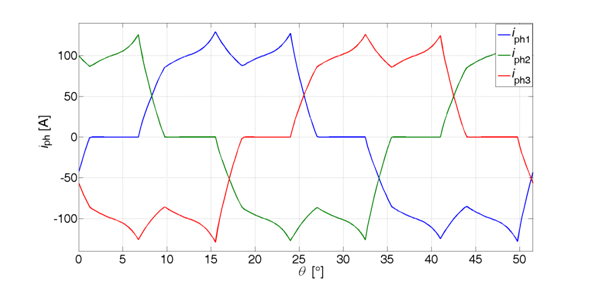
\includegraphics[width=12cm]{figures/fig2.png}
	\caption{Tytuł rysunku, rozmiar 11 pkt., pojedyncza interlinia, akapit wyśrodkowany, bez wcięcia pierwszego wiersza. Na końcu tytułu rysunku/tabeli nie stawia się kropki [8]}
	\label{Fig:wykres}
\end{figure}


\begin{example}
	[\ldots] oraz indukcyjności wzajemnej. W tabeli \ref{Tab:tabela} przedstawiono podstawowe parametry obwodu nieliniowego, zasilanego napięciem trójfazowym.
\end{example}

\begin{table}[ht]
	\caption{Tytuł tabeli, rozmiar 11 pkt., pojedyncza interlinia, akapit wyrównany do lewej}
	\centering
	\begin{tabular}{|c|c|c|c|c|}
		\hline
		$U$ [V] & $I$ [mA] & $R$, [k$\Omega$] & $L$ [mH] & $R/R_{20}$ \\
		\hline
		13,6    & 7,29     & 3,94             & 100      & 1,25       \\
		\hline
	\end{tabular}

	\label{Tab:tabela}
\end{table}

{\subsubsection{Wzory matematyczne}}

Zmienne we wzorach pisze się czcionką pochyłą (styl edytora równań „Matematyka”) natomiast symbole, nie będące zmiennymi, czcionką prostą (styl „Tekst”).
Rozmiary czcionek: normalny 12 punktów, indeks dolny/górny 9 pkt., indeks podrzędny 7 pkt., symbol 24 pkt., podsymbol 12 pkt. Separatorem dziesiętnym w liczbach jest
przecinek, a nie kropka (dotyczy to również liczb pisanych w tekście akapitu). Poddaj się w tym zakresie \LaTeX'owi - pisz wzór, a poprawnie się utworzy.


Pod wzorem należy zamieścić objaśnienia użytych symboli (chyba, że znajdują się w wykazie na początku pracy). Wzory umieszcza się wyśrodkowane i numeruje zgodnie
z kolejnością w danym rozdziale: (numer\_rozdziału.numer\_wzoru). Numery wzorów wyrównuje się do prawego marginesu. W akapicie poprzedzającym wzór musi znajdować się krótki opis, czego dotyczy dany wzór i – jeżeli potrzeba – odwołanie do literatury.

\begin{example}
	[\ldots] wyznacza się, na podstawie wyrażenia (\ref{Eq:rownanie}). W nawiasach podano rozmiary czcionek używanych we wzorach
\end{example}

\begin{equation}
	A(12)={\sum}(24)m_{s(9)}N^{k_{p(7)}}
	\label{Eq:rownanie}
\end{equation}
gdzie: $m_s$ -- masa próbki, $N$ -- natężenie oświetlenia, $k_p$ -- wykładnik potęgi $(k_p=1,3-2,1)$.\\
\newpage
{\subsubsection{Listingi programów}}

W pracy dyplomowej możesz umieszczać fragmenty programów. Pamiętaj, aby umieszczać krótkie, tylko najważniejsze fragmenty kodów źródłowych. Zawsze je komentuj w treści
pracy dyplomowej. Typowo w \LaTeX\ kody źródłowe umieszczane są w środowisku verbatim (\verb|\begin{verbatim}...\end{verbatim}|). Obecnie instnieje jednak bardziej nowoczesne i bardziej funkcjonalne środowisko \verb|lstlisting| (wymaga zainstalowanego w systemie pakietu \verb|listings|). Zwróć uwagę, że możesz kolorować składnię
automatycznie za pomocą parametru \verb|language|. W niniejszym dokumencie przedstawiono dwa przykłady listingów, Listing \ref{KodMatlab1} to przykład kodu źródłowego Matlaba, a poniżej Listing \ref{KodPerl1} dla Perl'a.\\
%\komentarz{

\begin{lstlisting}[language=Matlab,caption=Listing programu Matlab,label={KodMatlab1}]
i = 1
p = 3
for i = 1:10
    if i > 3
        i=i+p
    else 
        i=i+1
    end
end
\end{lstlisting}

\begin{lstlisting}[language=Python,caption=Listing programu Perl,label={KodPerl1}]
  my $url ='http://pei.prz.edu.pl';
  use LWP::Simple;
  my $content = get $url;
  die "Couldn't get $url" unless defined $content;
  print $content;
  print "\n";
  print "Length " + length($content)
\end{lstlisting}

Z pewnością przeglądając źródło tego dokumentu zobaczysz, że kody źródłowe powinny mieć zdefiniowane parametry \verb|label|, aby łatwo w tekście do nich się odwoływać.
Numeracja linii jest w stylu domyślnie włączona (to przydatne, bo w treści pracy łatwo odwołać się dzięki temu do konkretnego wiersza w kodzie źródłowym), możesz je wyłączyć podając jako parametr \verb|numbers=none|. Więcej szczegółów możesz odnaleźć w sekcji \verb|\lstset| pliku arkusza styli.
%}


\subsubsection{Numerowanie i punktowanie}

\begin{enumerate}[label=\arabic*), leftmargin=1.25cm]
	\item Pierwszy poziom (stosuje się numerowanie lub punktowanie). Formatowanie:
	      akapit wyjustowany, wcięcie od lewej 0,75 cm, wysunięcie co 0,5 cm.
	\item Znakiem numerowania jest liczba (z kropką lub nawiasem).
	      \begin{itemize}[label=-,labelsep=0.4cm,leftmargin=0.6cm]
		      \item drugi poziom (stosuje się wyłącznie punktowanie). Formatowanie: akapit
		            wyjustowany, wcięcie od lewej 1,25 cm, wysunięcie co 0,5 cm,
		      \item znakiem punktowania jest łącznik lub mała litera alfabetu (z nawiasem). Nie
		            zaleca się stosowania kropek, strzałek itp.,
		      \item punktowane akapity rozpoczyna się minuskułą (małą literą), na końcu akapitu
		            stawia się przecinek, ostatni punktowany akapit kończy się kropką.
	      \end{itemize}
	\item Numerowane akapity rozpoczyna się majuskułą (wielką literą) i kończy kropką.
	\item Należy zwrócić uwagę, aby nie rozdzielać numerowania/punktowania pomiędzy
	      kolejnymi stronami tekstu.
\end{enumerate}


\subsection{Wykaz literatury}

W wykazie literatury zamieszcza się wyłącznie pozycje, na które powołano się
w pracy. Kolejność numerów w wykazie – zgodna z kolejnością pojawiania się danej
pozycji w tekście.

Format akapitu: akapit wyjustowany, wysunięcie 0,75 cm. Prawidłowo opracowany
wykaz został zaprezentowany w niniejszym dokumencie w odpowiednim rozdziale, oznaczonym jako „Literatura”  (pozycja nr \cite{str} to zasoby internetowe,
\cite{Jakubczyk1997} – książka, \cite{Barski2011} – artykuł w czasopiśmie, \cite{dokum} – karta katalogowa).

	{\subsection{Wydruk pracy}}

Przed wydrukiem należy usunąć ewentualne błędy literowe i sprawdzić prawidłową
interpunkcję. Przykładowo, łącznik zapisuje się za pomocą krótkiego minusa (np.
badawczo-rozwojowy) natomiast myślnik -- stosowany w zdaniach wtrąconych -- zapisuje
się za pomocą długiej pauzy. Dzielenie wyrazów według uznania Autora (można podzielić
długie wyrazy, powodujące duże „rozstrzelenie” tekstu w poprzedzającym wierszu. Zaleca się usunięcie pojedynczych znaków na końcu wiersza oraz podwójnych spacji w tekście.
Dla przedrostka „mikro” należy unikać stosowania litery „u” zamiast „$\mu$”. Znak „$\mu$” można
otrzymać przytrzymując lewy Alt i wpisując na klawiaturze numerycznej 0181 (podobnie
„stopień”: Alt-0176). W celu uniknięcia „rozstrzelenia” liczb i ich jednostek zaleca się
używanie „twardej” spacji pomiędzy liczbą i jednostką. Należy sprawdzić, czy tytuły
podrozdziałów/zakresów nie zostały jako pojedyncze wiersze na poprzedniej stronie oraz
czy rysunki/tabele i ich tytuły nie zostały rozdzielone pomiędzy kolejnymi stronami.

Pracę drukuje się dwustronnie. Zaleca się wydruk w kolorze. Przed wydrukiem
należy ponumerować strony (czcionka 10 pkt., dół strony, akapit wyśrodkowany). Strony
tytułowej oraz strony z podziękowaniem nie numeruje się. Spis treści rozpoczyna się od
strony numer 3 (lub 5, jeżeli zamieszczono podziękowania).

\clearpage

\section{Podsumowanie i wnioski końcowe}

1 $\div$ 3 stron merytorycznie podsumowanie najważniejszych elementów pracy oraz wnioski wynikające z osiągniętego celu pracy. Proponowane zalecenia i modyfikacje oraz rozwiązania będące wynikiem realizowanej pracy.

Ostatni akapit podsumowania musi zawierać wykaz własnej pracy dyplomanta i zaczynać się od sformułowania: „Autor za własny wkład pracy uważa: \ldots”.

\clearpage

\section*{Załączniki}
\addcontentsline{toc}{section}{Załączniki}

Według potrzeb zawarte i uporządkowane uzupełnienie pracy o dowolny materiał źródłowy (wydruk programu komputerowego, dokumentacja kons\-truk\-cyj\-no-\-tech\-no\-lo\-gicz\-na, konstrukcja modelu -- makiety -- urządzenia, instrukcja obsługi urządzenia lub stanowiska laboratoryjnego, zestawienie wyników pomiarów i obliczeń, informacyjne materiały katalogowe itp.).


\clearpage

\addcontentsline{toc}{section}{Literatura}

\begin{thebibliography}{4}
	\bibitem{str} http://weii.portal.prz.edu.pl/pl/materialy-do-pobrania. Dostęp 5.01.2015.
	\bibitem{Jakubczyk1997} Jakubczyk T., Klette A.: Pomiary w akustyce. WNT, Warszawa 1997.
	\bibitem{Barski2011} Barski S.: Modele transmitancji. Elektronika praktyczna, nr 7/2011, str. 15-18.
	\bibitem{dokum} Czujnik S200. Dokumentacja techniczno-ruchowa. Lumel, Zielona Góra, 2001.
	\bibitem{Pawluk2001} Pawluk K.: Jak pisać teksty techniczne poprawnie, Wiadomości Elektrotechniczne, Nr 12, 2001, str. 513-515.
\end{thebibliography}

\clearpage

\makesummary

\end{document}
